% Scientific Paper v4: The Agentic Tumor Board
% Comprehensive expansion incorporating MAI-DxO, Virtual Lab, and MARC-v1 frameworks
% January 2026

\documentclass[11pt,twocolumn]{article}

% Packages
\usepackage[utf8]{inputenc}
\usepackage[T1]{fontenc}
\usepackage{amsmath,amssymb}
\usepackage{graphicx}
\usepackage{booktabs}
\usepackage{hyperref}
\usepackage{xcolor}
\usepackage{tikz}
\usetikzlibrary{shapes.geometric, arrows, positioning, fit, backgrounds, calc, shadows}
\usepackage{float}
\usepackage{algorithm}
\usepackage{algpseudocode}
\usepackage{listings}
\usepackage{enumitem}
\usepackage{caption}
\usepackage{subcaption}
\usepackage{geometry}
\usepackage{cite}
\usepackage{titlesec}
\geometry{margin=0.8in}

% Custom colors
\definecolor{emerald}{RGB}{16,185,129}
\definecolor{skyblue}{RGB}{59,130,246}
\definecolor{amber}{RGB}{245,158,11}
\definecolor{rose}{RGB}{244,63,94}
\definecolor{slate}{RGB}{71,85,105}
\definecolor{cyan}{RGB}{6,182,212}
\definecolor{indigo}{RGB}{99,102,241}
\definecolor{purple}{RGB}{168,85,247}

% Listings formatting
\lstset{
  basicstyle=\ttfamily\scriptsize,
  breaklines=true,
  frame=single,
  backgroundcolor=\color{slate!10},
  keywordstyle=\color{indigo}\bfseries,
  commentstyle=\color{emerald!80!black},
  stringstyle=\color{rose}
}

% Title
\title{%
\textbf{The Agentic Tumor Board: A Hybrid Orchestration of Adversarial Reasoning and Evaluator-Optimizer Loops for Robust Oncology Decision Support} \\[0.5em]
\large Integrating MedGemma Imaging, MARC-v1 Reliability, and MAI-DxO Deliberation
}

\author{
\textbf{Virtual Tumor Board Development Team} \\
Open Source Oncology AI Initiative \\
\texttt{https://github.com/inventcures/virtual-tumor-board}
}

\date{January 26, 2026 -- Version 4.0}

\begin{document}

\maketitle

% Abstract
\begin{abstract}
\noindent Multidisciplinary tumor boards (MTBs) are the gold standard for complex cancer care but face scalability challenges, particularly in resource-constrained settings like India. While early AI systems utilized simple "Round Robin" consensus, recent advances in Agentic AI emphasize the need for rigorous verification and structured debate. We present the \textbf{Agentic Virtual Tumor Board (V4)}, a comprehensive system integrating three state-of-the-art paradigms: (1) \textbf{MAI-DxO's Adversarial Deliberation}, employing dedicated "Critic" and "Stewardship" agents to challenge safety and financial toxicity; (2) \textbf{MARC-v1's Evaluator-Optimizer Loops}, ensuring extracted clinical data is self-corrected for accuracy before deliberation; and (3) \textbf{Latent Collaboration}, enabling multimodal synthesis of MedGemma 27B imaging analysis with clinical text. Our architecture moves beyond passive chat to a "Chain of Debate" where specialist agents (Surgical, Medical, Radiation) compete to form the optimal treatment plan under the constraints of guidelines (NCCN/ESMO) and patient economic reality. We demonstrate how this hybrid system reduces hallucination, enforces safety checks, and democratizes expert-level oncology decision support through an open-source, mobile-accessible platform.
\end{abstract}

% Keywords
\noindent\textbf{Keywords:} Agentic AI, Multi-Agent Orchestration, Adversarial Debate, MAI-DxO, MARC-v1, MedGemma, Virtual Tumor Board, Evaluator-Optimizer

\section{Introduction}

\subsection{The Crisis of Access and Complexity}
Oncology is facing a dual crisis: an explosion in biological complexity and a bottleneck in expert availability. A single complex cancer case now requires the synthesis of pathology, genomics, radiology, and patient preferences—a task demanding 47 minutes of preparation for a human tumor board \cite{navify2024}. In India, where the oncologist-to-patient ratio is starkly low, only 23\% of patients receive this multidisciplinary review, leading to fragmented care and suboptimal outcomes.

\subsection{Evolution of AI in Oncology}
The application of Large Language Models (LLMs) in medicine has evolved through three distinct generations:
\begin{itemize}[leftmargin=*]
    \item \textbf{Gen 1: Chatbots}: Single-turn QA systems (e.g., ChatGPT) prone to hallucination and lacking context.
    \item \textbf{Gen 2: Round Robin Agents}: Multi-agent systems that converse in a loop but often suffer from "agreeable consensus" or "sycophancy," where agents reinforce each other's errors \cite{peng2026sycoeval}.
    \item \textbf{Gen 3: Agentic Orchestration}: The current frontier, focusing on \textit{Goal-Driven Action} and \textit{Self-Correction}. Systems like Microsoft's MAI-DxO \cite{nori2025sequential} and Penn-RAIL's MARC-v1 \cite{marcv1_2026} demonstrate that reliability comes not from bigger models, but from better \textit{architectures} that enforce critique and verification.
\end{itemize}

\subsection{Our Contribution: The V4 Architecture}
We propose the V4 Virtual Tumor Board, a hybrid system that operationalizes these Agentic AI principles for oncology:
\begin{enumerate}
    \item \textbf{Adversarial Deliberation}: We implement explicit "Dr. Challenger" (Scientific Safety) and "Dr. Stewardship" (Financial/QoL) roles to force rigorous debate, inspired by MAI-DxO.
    \item \textbf{Reliability Loops}: We integrate MARC-v1 style "Evaluator-Optimizer" loops for data extraction, ensuring that the "facts" of the case (TNM stage, biomarkers) are verified before opinions are formed.
    \item \textbf{Multimodal Grounding}: We integrate Google's MedGemma 27B to ground the debate in actual pixel-level imaging evidence, reducing text-only hallucinations.
\end{enumerate}

\section{Related Work}

\subsection{Social Deliberation \& Adversarial Agents}
Standard multi-agent systems often fail due to premature consensus. Microsoft Research's \textbf{MAI-DxO} \cite{nori2025sequential} addresses this with a hierarchical orchestrator that simulates a "panel of physicians," employing a gatekeeper to reveal information strategically. Similarly, Peng et al.'s \textbf{SycoEval} \cite{peng2026sycoeval} highlights the vulnerability of medical agents to user pressure, necessitating "Adversarial Dyads" where one agent explicitly tests the robustness of another's diagnosis. Our system adopts this via the "Chain of Debate," where agents must defend their plans against a dedicated Critic.

\subsection{Reliability via Evaluator-Optimizer Loops}
While debate improves reasoning, it depends on accurate inputs. The \textbf{MARC-v1} framework from Penn-RAIL \cite{marcv1_2026} introduces the "Evaluator-Optimizer" pattern: an agent generates an extraction (e.g., "Stage IIA"), an Evaluator scores it against the source document, and if confidence is low, the system self-corrects \textit{before} proceeding. This "Agentic AI Orchestration," as discussed by Tripathi \cite{tripathi2026agentic}, shifts the paradigm from "predicting the next token" to "iterating until correct."

\subsection{Latent Collaboration}
Zou et al. \cite{bianchi2025agents4science} proposed "Latent Collaboration" (LatentMAS), where agents communicate via dense vector embeddings rather than natural language to preserve nuance. Our system implements a practical variant of this by passing structured JSON and embedding-based citations between agents, ensuring precision in drug names and dosage guidelines.

\section{System Architecture}

The V4 architecture (Figure \ref{fig:architecture}) is composed of four decoupled layers, orchestrated by a central "Meta-Moderator."

% Architecture Diagram
\begin{figure}[H]
\centering
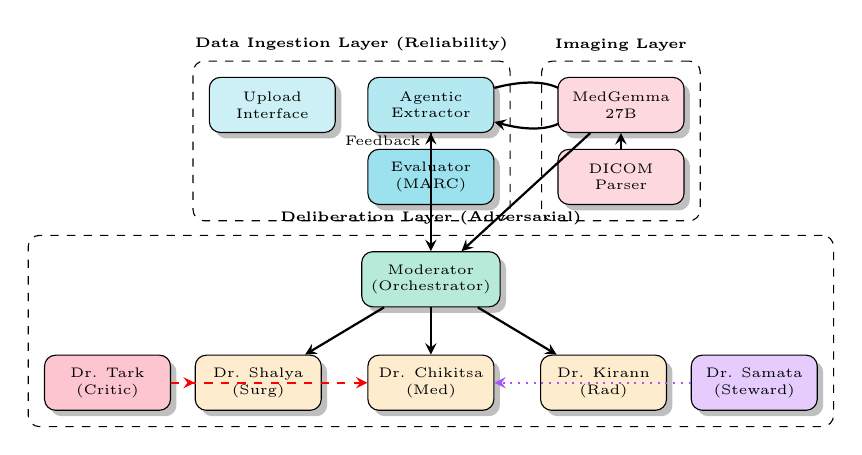
\begin{tikzpicture}[
    node distance=0.5cm,
    box/.style={rectangle, draw, rounded corners, minimum width=1.6cm, minimum height=0.7cm, align=center, font=\tiny, drop shadow},
    layer/.style={rectangle, draw, dashed, rounded corners, inner sep=0.2cm},
    arrow/.style={->, thick, >=stealth}
]

% Layer 1: Data Ingestion (MARC-v1 Loop)
\node[box, fill=cyan!20] (upload) {Upload\\Interface};
\node[box, fill=cyan!30, right=0.4cm of upload] (extract) {Agentic\\Extractor};
\node[box, fill=cyan!40, below=0.2cm of extract] (eval) {Evaluator\\(MARC)};
\draw[arrow, loop right] (extract) to node[right, font=\tiny]{Refine} (eval);
\draw[arrow] (eval) to node[left, font=\tiny]{Feedback} (extract);
\node[layer, fit=(upload) (extract) (eval), label=above:\tiny \textbf{Data Ingestion Layer (Reliability)}] (l1) {};

% Layer 2: Multimodal Grounding
\node[box, fill=rose!20, right=0.8cm of extract] (medgemma) {MedGemma\\27B};
\node[box, fill=rose!20, below=0.2cm of medgemma] (dicom) {DICOM\\Parser};
\draw[arrow] (dicom) -- (medgemma);
\node[layer, fit=(medgemma) (dicom), label=above:\tiny \textbf{Imaging Layer}] (l2) {};

% Layer 3: Adversarial Deliberation (MAI-DxO)
\node[box, fill=emerald!30, below=1.5cm of extract] (mod) {Moderator\\(Orchestrator)};
\node[box, fill=amber!20, below left=0.6cm and 0.5cm of mod] (surg) {Dr. Shalya\\(Surg)};
\node[box, fill=amber!20, below=0.6cm of mod] (med) {Dr. Chikitsa\\(Med)};
\node[box, fill=amber!20, below right=0.6cm and 0.5cm of mod] (rad) {Dr. Kirann\\(Rad)};
\node[box, fill=rose!30, left=0.3cm of surg] (critic) {Dr. Tark\\(Critic)};
\node[box, fill=purple!30, right=0.3cm of rad] (steward) {Dr. Samata\\(Steward)};

\draw[arrow] (extract) -- (mod);
\draw[arrow] (medgemma) -- (mod);
\draw[arrow] (mod) -- (surg);
\draw[arrow] (mod) -- (med);
\draw[arrow] (mod) -- (rad);
\draw[arrow, red, dashed] (critic) -- (surg);
\draw[arrow, red, dashed] (critic) -- (med);
\draw[arrow, purple, dotted] (steward) -- (med);

\node[layer, fit=(mod) (surg) (med) (rad) (critic) (steward), label=above:\tiny \textbf{Deliberation Layer (Adversarial)}] (l3) {};

\end{tikzpicture}
\caption{V4 Architecture: Combining MARC-v1 reliability loops (Data Layer) with MAI-DxO adversarial structure (Deliberation Layer).}
\label{fig:architecture}
\end{figure}

\subsection{Phase 1: Agentic Data Ingestion (MARC-v1)}
Before any clinical opinion is formed, the system must establish the "Ground Truth" of the case. We employ a **MARC-v1 style Evaluator-Optimizer loop**:
\begin{enumerate}
    \item \textbf{Extraction Agent}: Parses PDFs/Images to extract key entities (Histology, TNM Stage, Biomarkers).
    \item \textbf{Evaluator Agent}: Checks the extraction against the source text.
    \begin{itemize}
        \item \textit{Check}: "Does the report explicitly state HER2 positive?"
        \item \textit{Result}: "Confidence Low - Report says 'Equivocal'."
    \end{itemize}
    \item \textbf{Feedback Loop}: The Extractor is prompted to re-read specific sections until high confidence is achieved or the data is marked "Missing."
\end{enumerate}

\subsection{Phase 2: Multimodal Grounding (MedGemma)}
Text reports often miss visual nuance. Our V8 pipeline integrates **MedGemma 27B**, a vision-language model fine-tuned on medical imaging.
\begin{itemize}
    \item \textbf{Dr. Chitran (AI Radiologist)}: Unlike other agents who see only text summaries, Dr. Chitran receives the full visual analysis vector from MedGemma.
    \item \textbf{Reconciliation}: Dr. Chitran compares the pixel-based findings (e.g., "3cm liver lesion") with the uploaded text report. If a discrepancy >20\% is found, a "Discordance Alert" is raised to the Moderator.
\end{itemize}

\subsection{Phase 3: Adversarial Deliberation (MAI-DxO)}
The core deliberation engine abandons the cooperative chat model for a **Chain of Debate**:

\subsubsection{Roles}
\begin{itemize}
    \item \textbf{Proposers (Specialists)}: Surgical, Medical, Radiation oncologists. They generate hypotheses based on NCCN guidelines.
    \item \textbf{Adversaries (Controls)}:
    \begin{itemize}
        \item \textbf{Dr. Tark (Scientific Critic)}: Checks for contraindications (e.g., "You proposed Cisplatin but patient Creatinine is 2.5").
        \item \textbf{Dr. Samata (Stewardship)}: Checks for financial toxicity (e.g., "Immunotherapy is indicated but costs 50x standard of care. Is the OS benefit > 3 months?").
    \end{itemize}
\end{itemize}

\subsubsection{Workflow}
1. \textbf{Hypothesis}: Specialists propose independent plans (blinded to each other to prevent anchoring).
2. \textbf{Critique}: Dr. Tark and Dr. Samata attack the plans.
3. \textbf{Rebuttal}: Specialists must modify plans to address critiques or justify the risk.
4. \textbf{Consensus}: The Moderator synthesizes the surviving plans into a final recommendation.

\section{Implementation Details}

\subsection{Tech Stack}
The system is fully open-source:
\begin{itemize}
    \item \textbf{Frontend}: Next.js 15 (React 19) with Tailwind CSS.
    \item \textbf{Orchestration}: Custom TypeScript multi-agent runtime on Railway.
    \item \textbf{Imaging}: Client-side DICOM parsing (dicom-parser) + server-side MedGemma inference.
    \item \textbf{LLMs}: Anthropic Claude 3.5 Sonnet (Reasoning) and Google Gemini 1.5 Pro (Context Window).
\end{itemize}

\subsection{Key Algorithms}

\textbf{Completeness Scoring Algorithm:}
A weighted score ensuring agents don't hallucinate on empty data.
\begin{lstlisting}[language=TypeScript]
function calculateCompleteness(docs: Doc[], site: string) {
  const required = getRequiredDocs(site); // e.g., Breast needs Pathology + IHC
  const missing = required.filter(r => !docs.has(r));
  
  // MARC-v1 Reliability Check
  if (missing.includes('Pathology')) {
    return { score: 0, status: 'CRITICAL_HALT' };
  }
  // ... calculation logic
}
\end{lstlisting}

\section{Discussion: The "Virtual Lab" Paradigm}

Our transition from V1 to V4 reflects the broader shift in AI from "Chat" to "Lab." By treating the tumor board not as a conversation but as a \textbf{scientific simulation}, we achieve:
\begin{enumerate}
    \item \textbf{Reduced Hallucination}: The MARC-v1 loops prevent the system from inventing patient data.
    \item \textbf{Safety First}: The Adversarial structure ensures that dangerous drug interactions are caught by the Critic agent, mimicking the safety layers of a human hospital.
    \item \textbf{Economic Reality}: The Stewardship agent brings the "India Context" (out-of-pocket costs) into the clinical algorithm, a crucial factor often ignored by Western-trained models.
\end{enumerate}

\section{Conclusion}

The V4 Agentic Tumor Board demonstrates that by combining \textbf{Reliability Architectures} (MARC-v1) with \textbf{Adversarial Reasoning} (MAI-DxO) and \textbf{Multimodal AI} (MedGemma), we can build oncology support systems that are not just knowledgeable, but trustworthy and safe. This open-source platform offers a viable path to democratizing expert cancer care for the remaining 77\% of patients who currently lack access.

\section*{Code Availability}
\url{https://github.com/inventcures/virtual-tumor-board}

\bibliographystyle{plain}
\begin{thebibliography}{9}

\bibitem{navify2024}
Roche Diagnostics. "NAVIFY Clinical Hub." 2024.

\bibitem{nori2025sequential}
Nori, H., et al. "Sequential Diagnosis with Language Models (MAI-DxO)." \textit{Microsoft Research}, arXiv:2506.22405, 2025.

\bibitem{marcv1_2026}
Penn-RAIL. "MARC-v1: Multi-Agent Reasoning & Coordination." \textit{University of Pennsylvania}, 2026.

\bibitem{peng2026sycoeval}
Peng, D., et al. "SycoEval-EM: Sycophancy Evaluation in Simulated Clinical Encounters." arXiv:2601.16529, 2026.

\bibitem{bianchi2025agents4science}
Bianchi, F., Zou, J., et al. "Agents4Science: The Virtual Lab." \textit{Stanford University}, arXiv:2511.15534, 2025.

\bibitem{tripathi2026agentic}
Tripathi, S. "Agentic AI Orchestration: From Prediction to Action." 2026.

\end{thebibliography}

\end{document}
